%%%%%%%%%%%%%%%%%%%%%%%%%%%%%%%%%%%%%%%%%%%%%%%%%%%%%%%%%%%%%%%%%%%%%%%%
%                                                                      %
%     File: Thesis_Implementation.tex                                  %
%     Tex Master: Thesis.tex                                           %
%                                                                      %
%     Author: Francisco Mendes                                         %
%     Last modified :  28 Nov 2019                                     %
%                                                                      %
%%%%%%%%%%%%%%%%%%%%%%%%%%%%%%%%%%%%%%%%%%%%%%%%%%%%%%%%%%%%%%%%%%%%%%%%

\chapter{Proposal}
\label{chapter:implementation}
\begin{figure}[!htb]
  \centering
  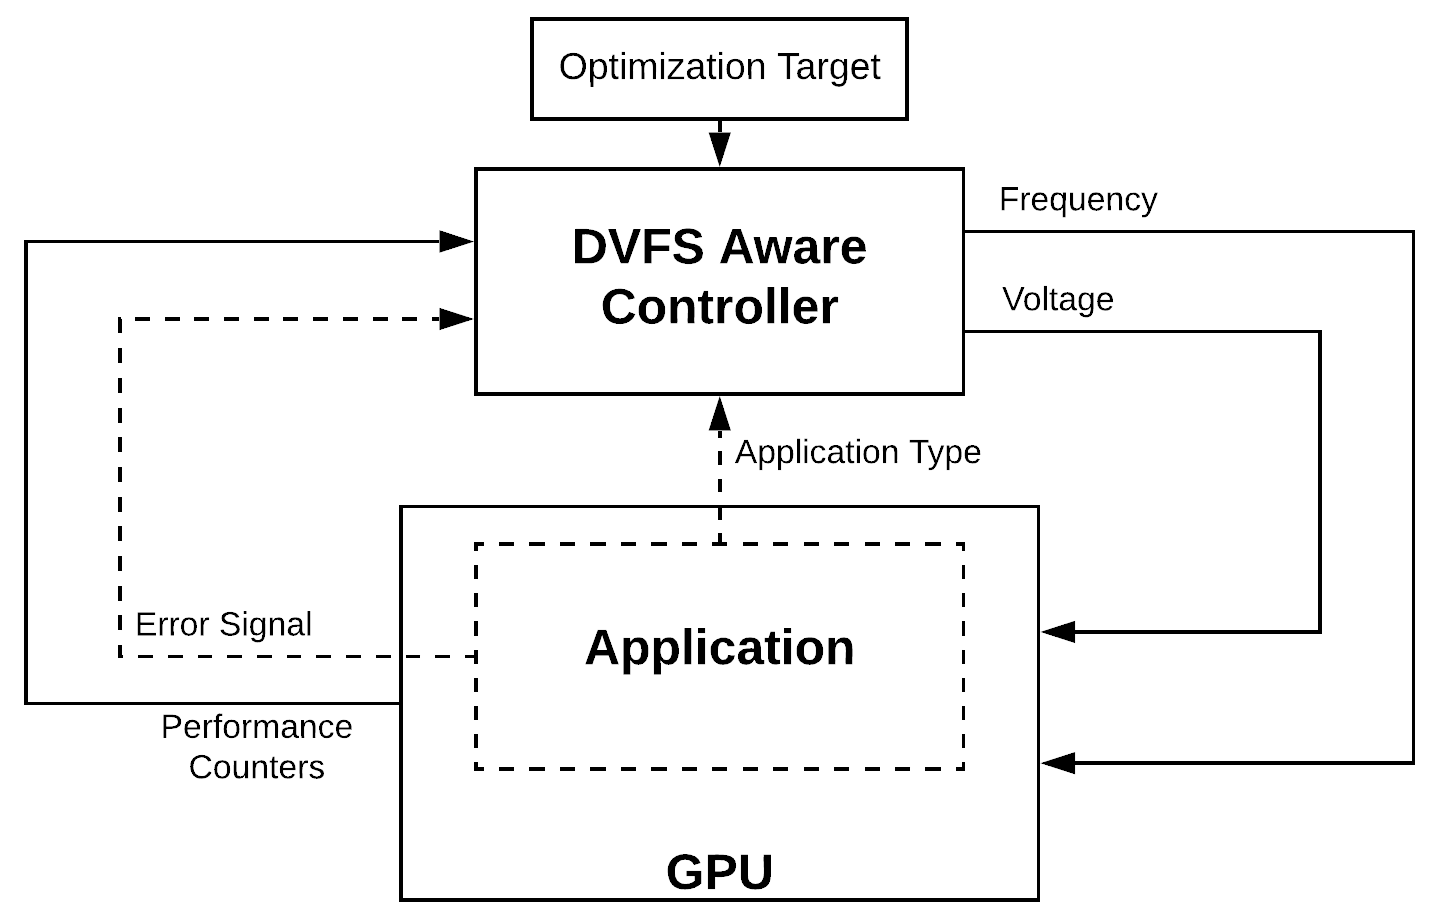
\includegraphics[width=0.75\textwidth]{Figures/Proposel/DVFS_Aware_Controller.png}
  \caption[Controller]{DVFS Aware Controller Block Diagram.}
  \label{fig:controlerDVFSaware}
\end{figure}

The main goal of this work is to designed and implement a GPU DVFS aware mechanism. This new mechanism will enforce non-conventional DVFS parameters to improve the energy efficiency of GPU devices, running deep learning applications. 

Two steps are required to acquire sufficient knowledge to design the controller. First, a characterization of the use of non-conventional DVFS parameters has to be performed for different workload scenarios, and second, a power and performance model has to be created. This chapter will start by providing an overview of how those two steps are going to be executed and what kinds of insights are expected to be uncovered. Then an overview of the GPU DVFS aware mechanism will be provided, connecting how do the previous points are connect, in the architecture of the solution. Finally, an overview of how the mechanism will be tested is described is presented.

The experimental work will be conducted on the Radeon Vega Frontier Edition presented in Chapter 2. This GPU provides the two necessary tools to both do the DVFS exploration and customization implementation through the profiling software - ROC-Profiler \cite{noauthor_rocm-developer-tools/rocprofiler_2019}, and tunning software - ROC-SMI \cite{noauthor_radeonopencompute/roc-smi_2019}.

\section{Non-convectional GPU DVFS characterization}

The objective of the characterization is to understand how the different workloads impact the voltage margin and how does performance and energy consumption relates to DVFS parameters. 

This part of the work will extend the work of Guerreiro \textit{et al.} in \cite{guerreiro_gpgpu_2018} \cite{guerreiro_modeling_2019} and Leng \textit{et al.} in \cite{leng_safe_2015}, by combining aggressive but safe voltage reduction with the
drawing of optimization curves, like the one of Figure \ref{fig:optcurves}. In this kind of plot, points of frequency/voltage are drawn, relating the performance achieved with the amount of energy spent. By using it, it is possible to optimize the DVFS settings for pure performance, energy efficiency or energy saving.

\begin{figure}[!htb]
  \centering
  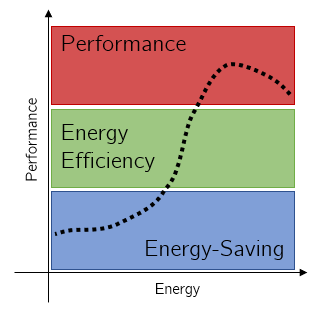
\includegraphics[width=0.3\textwidth]{Figures/Proposel/curves.png}
  \caption[Controller]{Example of optimization curve.}
  \label{fig:optcurves}
\end{figure}

The characterization will be done in two levels, first a fundamental analysis, using simple benchmarks, and at a higher level, using DNN primitives individually.

\subsection{Fundamental Analysis}
\label{sec:funAnali}
As stated in chapter 2, GPUs contain a significant voltage guardband to guarantee correct operation for all kinds of workloads and to be able to resist voltage noise. Using the benchmarks presented in Section \ref{sec:funAnal}, the size of these margins will be measured, first for each kind of benchmarks, and then to combinations of them, mimicking more complex workloads. This analysis will be performed by repeatedly running each benchmark at increasingly reduced voltage, and evaluating if the results being produced are the ones expected. When a benchmark is not able to be run at the indented under-voltage value, due to computation errors, or GPU crashes, the minimum voltage, $V_{min}$, is identified.

This analysis will allow an understanding of the impact that the activation and deactivation of the different GPU components cause on the voltage noise, the main contributing factor to the size of the voltage guardband.

The second part of the analysis is to create the optimization curves for each benchmark type and to comprehend what types of workloads have a dominant weight over $V_{min}$, performance and energy.


\subsection{DNN Primitives Analysis}
The insights of the fundamental analysis will help to guide the DNN primitive analysis and characterization. Here, the benchmarks proposed in Section \ref{sec:dnnPri} will be used to understand how to optimize the different layers of a complete DNN. 

On the preliminary work, Section 3.3, the $V_{min}$ was determined for a CNN; however, this results only indicates that there is a specific layer on that CNN that has the determined  $V_{min}$. The characterization of DVFS parameters in a per layer way allows for further optimizations of the DVFS to the running neural network.

\section{Power and Performance Model}
The second step to create the DVFS aware mechanism is to have a valid prediction model for power and performance. This mechanism will use the performance counters extracted from the runtime of the benchmarks from Section \ref{sec:funAnal} and ref{sec:dnnPri}, references for the type of application and user input of the desired optimization (performance, energy efficiency or energy saving) to predict $V_min$ and the best pair of frequency/voltage. Figure \ref{fig:model} exemplifies the block diagram of the power and performance model.

\begin{figure}[!htb]
  \centering
  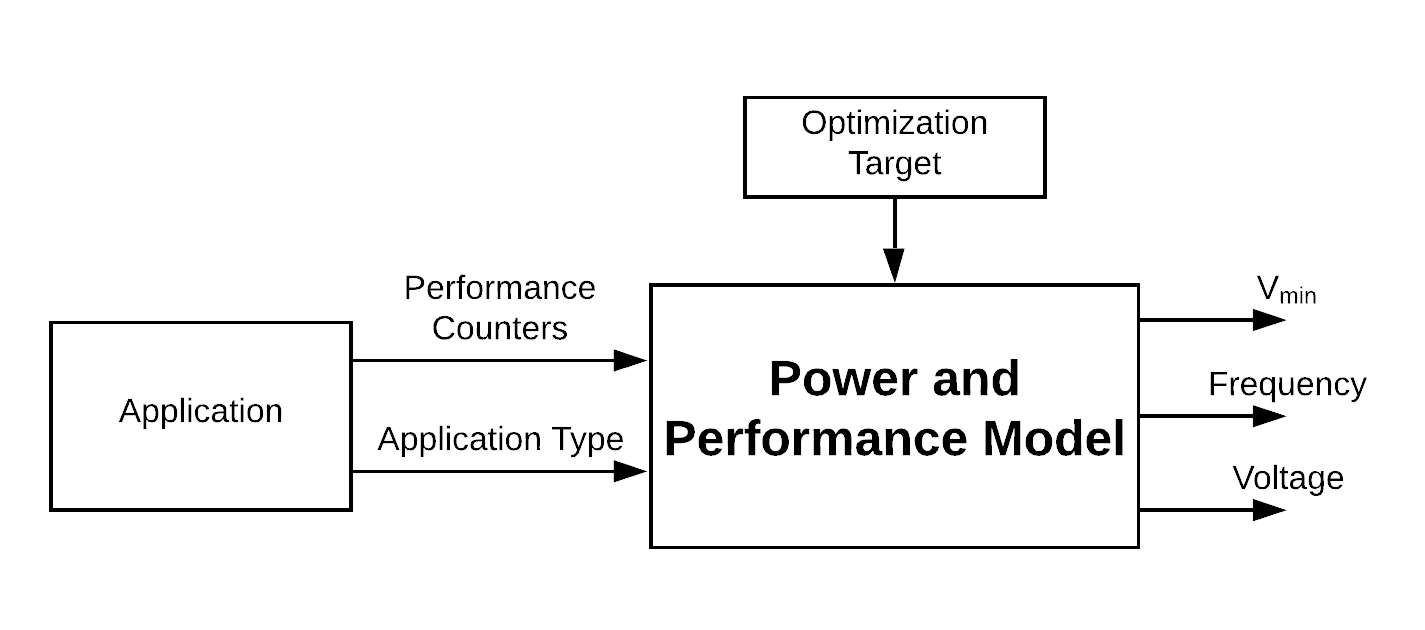
\includegraphics[width=0.8\textwidth]{Figures/Proposel/model.png}
  \caption[Controller]{Block Diagram of Power and Performance Model.}
  \label{fig:model}
\end{figure}. 

The profiling results from Section 4.1.1,  (performance counters values, performance, power and energy) will be used to train an artificial neural network (ANN) that will model the power and prediction. Following the approach of Song \textit{et al.} \cite{song_simplified_2013} and Guerreiro  \textit{et al.} \cite{guerreiro_modeling_2019}, the trained ANN should be able to correctly predict the best DVFS settings for both simple kernels, as well, for DNN primitives and full DNN layers from Section 4.1.2.

%%%%%%%%%%%%%%%%%%%%%%%%%%%%%%%%%%%%%%%%%%%%%%%%%%%%%%%%%%%%%%%%%%%%%%%%
\section{GPU DVFS Aware Mechanism}
\label{section:DVFSaware}

To design the controller, it is first necessary to extend the profiling application to support on-demand performance counters query and profiling of none C based applications. Since the deep learning libraries and applications used nowadays are developed in Python, a C static library will be developed, in order to have access to the performance counters values, at higher-level programming languages.

With an on-demand profiler, it is possible to construct a \textit{watch} application responsible for monitoring both the GPU and the deep learning application state. The \textit{watch} application will control the AMD DVFS mechanism, through the ROC-SMI interface, by providing the best frequency and voltage level for each performance level and by setting, depending on the DNN layer running, the most appropriated performance level, depending on the user optimization target (performance, energy efficiency or energy savings).



